\documentclass[twocolumn,a4paper,11pt]{article}
\usepackage[utf8]{inputenc}
\usepackage[T1]{fontenc}
\usepackage{amsmath}
\usepackage{amssymb}
\usepackage{graphicx}
\usepackage{xcolor}
\usepackage[margin=1.75cm]{geometry}
\usepackage{hyperref}

\bibliographystyle{ieeetr}

\newcommand{\citeme}{\textbf{\textcolor{red}{CITEME}}}

\author{Josh Pattman}
\title{Evolutionary Learning with Extended Mutation Techniques}
\begin{document}
	\maketitle
    \section{Introduction}
    Two of the most important features when describing an organism are its genotype and its phenotype. A genotype encompasses the entire genetic code of an organism, while the phenotype is the physical manifestation of that code as specific traits such as size or color. The relationship between a genotype and a phenotype is a complex one, as a single locus in the genotype does not hold a one-to-one relationship with a single trait in the phenotype. Instead, the phenotype is the result of the entire genotype interacting with the gene regulation network (GRN) of the organism.

    A GRN is a mechanism by which the various genes in the genotype interact by stimulating or repressing each other, eventually resulting in a stable state describing the phenotype \cite{what-is-grn}. This is an extremely complex process but has been simplified to a dense directed graph in previous research \cite{grn-1}. Each node in the GRN graph represents a locus in both the genotype and phenotype, and connections between nodes represent the interactions between genes.
    
    The topology of the GRN is not fixed throughout generations, but instead evolves alongside the genotypes of the organisms, with each organism having its own unique GRN \cite{evolving-grns}. However, the rate of evolution of the GRN is significantly slower than that of the genotype \cite{evo-speed-grn}, meaning that the GRN may retain information from previous fitness landscapes, even if that information is not immediately useful to a given organism at present \cite{grn-learn-from-past}.

    Evolved GRNs have several interesting properties. For example, a GRN may recognize genes that frequently covary, and increase the likelihood of those genes being expressed together. A GRN also may take advantage of its ability to retain information to increase the likelihood of a group of traits from a previous landscape being expressed in the future. This is particularly useful as a previously proven trait of a creature may be more helpful in a future environment than a new randomly evolved one. This ability of a GRN to remember previous fitness landscapes will be referred to as genetic memory throughout this research.

    This paper aims to investigate the effects of genetic memory in a variety of scenarios, building upon previous work by Richard A. Watson Et al. \cite{original-paper}, henceforth referred to as the previous work. In the previous work, a specific mathematical model for a genotype and GRN was created, and a hill-climbing algorithm was performed to optimize a GRN to commit multiple phenotypes to memory. The trained GRN was then used to produce various combinations of the training phenotypes upon being presented with a random genotypic input.

    The previous work also showed that using their specific method, the weights of the GRN tended to move towards the weights achieved by Hebbian learning on the training data. This result is significant, as it suggests a hill climbing algorithm may in part be equivalent to more traditional 'intelligent' machine learning algorithms.

    This paper aims to initially reimplement the algorithms of the previous work, and reproduce the results obtained. Following this, an extension to the previous work is proposed, which aims to more accurately model the mutations applied to a GRN. This extension is then extensively tested and the results are compared to the original work.

    \section{Experiment Setup}
    To represent the genotype of an organism, a vector $G$ is used. This vector has one element per gene in the organism, which in many of the presented cases is visualized by a pixel in an image. Each element can be any in the range $[-1,1]$.

    The GRN is represented by an interaction matrix $B$, which has the same number of rows and columns as there are elements in $G$. The state of the GRN at time $t$ is represented by a vector $P(t)$, which is governed by Equations \ref{eq:origpa} and \ref{eq:origp}. $P(t)$ has no upper and lower bound.
    
    \begin{equation} \label{eq:origpa}
        P(1) = G
    \end{equation}
    \begin{equation} \label{eq:origp}
        P(t+1) = P(t) + \tau_1 \sigma (B P(t)) - \tau_2 P(t)
    \end{equation}
    The symbols $\tau_1$ and $\tau_2$ represent the update rate and decay rate of the network respectively, and $\sigma$ is the $tanh$ function. The final phenotype on which the fitness is evaluated is given by $P(t_{final})$, where $t_{final}$ is set to 10 for all experiments in this paper.

    The fitness function of a GRN for a given target is formalized in Equation \ref{eqn:fitness}, which is a modified version of that used by the original work.
    \begin{equation} \label{eqn:fitness}
        |{sum} (P(t_{final}) \odot T)|
    \end{equation}
    In this equation, $T$ is the target phenotype and $\odot$ is the element-wise multiplication operator. Using this function, a value of 0 is minimally fit, but the fitness can extend to positive infinity. The reason for taking the absolute is that a perfect negative of the produced phenotype is indistinguishable from the target phenotype for the GRN. In the previous work, the fitness function would penalize a perfect negative, however this paper chooses to reward it.

    The genetic algorithm (GA) used in this paper is a simple point mutation hill-climbing model. At any given time step, there exist two individuals. One of these represents the previous best individual, and the other is a mutated version of the previous best. At each step, the mutated individual is re-initialized to the previous best, then a random point mutation is applied to both its genotype and GRN. If the mutated individual has a higher fitness than the previous best, it becomes the new previous best. This process is repeated for a set number of iterations, and the final best individual is returned. The point mutation size of the GRN must be significantly smaller than that of the genotype, otherwise the GRN may overwrite previously learned information. Mutations are uniformly distributed random numbers that are added to the previous value of the gene.

    \section{Reimplemented Results}
    To ensure that the simulation matched the original work, two of the original experiments were implemented. However, an in-depth analysis of these experiments is out-of-scope for this report, which instead favors detailed testing of the extension.

    \subsection{Two-Target GRNs} \label{sec:ttgrn}
    The primary goal of this experiment was to validate the implementation of the model of a GRN. It would achieve this by showing that the GRN was capable of committing multiple phenotypes to memory and recalling them in future iterations. It would also compare the results to the original work, ensuring that similar results were discovered.

    This experiment involved training the GRN based on two target phenotypes: $++---+-+$ and $+-+-+---$. Table \ref{tbl:ex-ttgrn-param} presents the parameters used in this experiment.

    \begin{table}[h]
        \centering
        \begin{tabular}{l|l}
        Parameter & Value \\ \hline
        $G$ Mutations & Uniform[-0.1:0.1] \\
        $B$ Mutations & Uniform[-0.0067:0.0067] \\
        Generations & 80000 \\
        Target Switch Each & 2000 \\
        $\tau_1$ & 1.0 \\
        $\tau_2$ & 0.2 \\
        $t_{final}$ & 10
        \end{tabular}
        \caption{The parameters of the Two-Target experiment.} \label{tbl:ex-ttgrn-param}
    \end{table}

    Figure \ref{fig:2a} shows how various values of the GRN matrix change throughout the iterations of training. Each value is represented by a line, with the x-axis representing the generation number and the y-axis representing the value of the $B$ matrix. It is clear to see that there are three distinct groups of parameters: increasing, decreasing, and static. The increasing and decreasing groups are due to the GRN learning either a positive or negative correlation between the genes that it connects, whereas the static group is due to the GRN learning that the genes are not correlated. The results are very similar to that of the original paper.
    \begin{figure}[h]
        \centering
        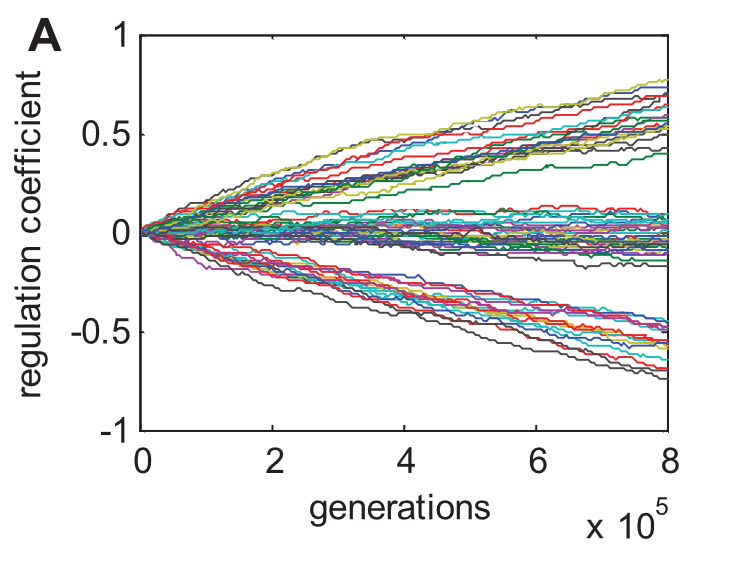
\includegraphics[width=0.48\linewidth]{orig_img/fig2a.png}
        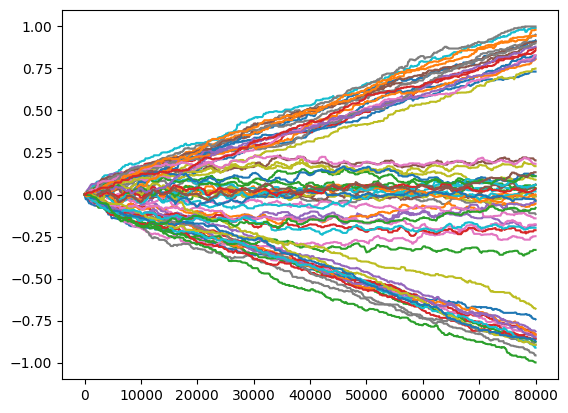
\includegraphics[width=0.48\linewidth]{img/fig2a.png}
        \caption{Values in $B$ over generations. On the left is the original paper. On the right is the reimplemented result.} \label{fig:2a}
    \end{figure}

    Figure \ref{fig:2b} visualizes the matrix $B$ at the end of training. An identical pattern of positive and negative values to that of the original paper emerged. However, the weights have a different scale, likely due to small changes in the implementation such as mutation rate. Similarly, Figure \ref{fig:2c} shows the weights obtained using Hebbian learning for $B$. As expected, the weights are very similar to those obtained through hill climbing, suggesting that the hill climbing algorithm may approximate Hebbian learning in this situation.

    \begin{figure}[h]
        \centering
        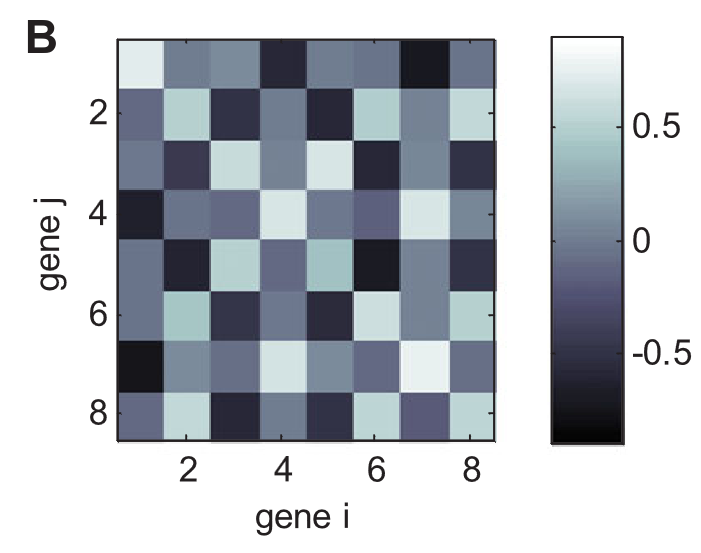
\includegraphics[width=0.48\linewidth]{orig_img/fig2b.png}
        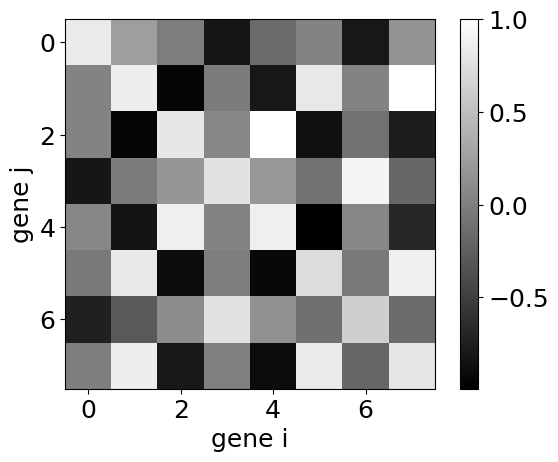
\includegraphics[width=0.48\linewidth]{img/fig2b.png}
        \caption{The final weights in $B$ obtained through a hill climbing process. On the left is the original paper. On the right is the reimplemented result.} \label{fig:2b}
    \end{figure}

    \begin{figure}[h]
        \centering
        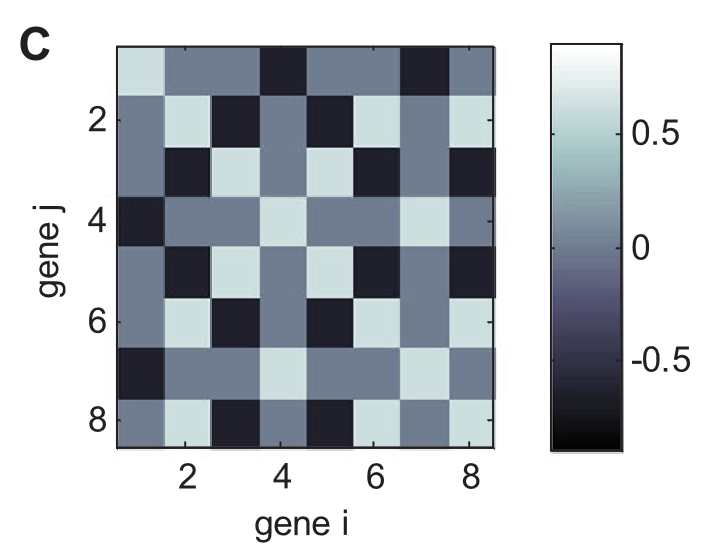
\includegraphics[width=0.48\linewidth]{orig_img/fig2c.png}
        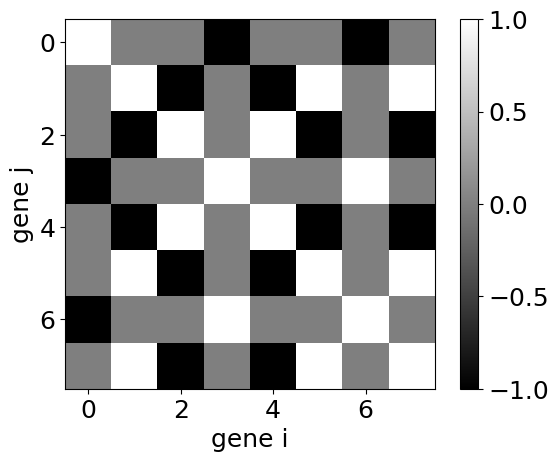
\includegraphics[width=0.48\linewidth]{img/fig2c.png}
        \caption{The weights obtained using Hebbian learning for $B$. On the left is the original paper. On the right is the reimplemented result.} \label{fig:2c}
    \end{figure}

    Figure \ref{fig:2d} demonstrates how the values of $P$ change over the 10 developmental timesteps. Each gene in $P$ is represented by a line, with the x-axis representing the developmental timestep and the y-axis representing the value of the gene. The results presented by this paper mirror those from the original work, with the genes all converging to either a stable positive or negative state by the end of the 10 timesteps. There is some correlation between a gene's starting value and the state it finally ends up in but Figure \ref{fig:2d} shows that is not the exclusive deciding factor, with some genes clearly changing signs from their original value.

    \begin{figure}[h]
        \centering
        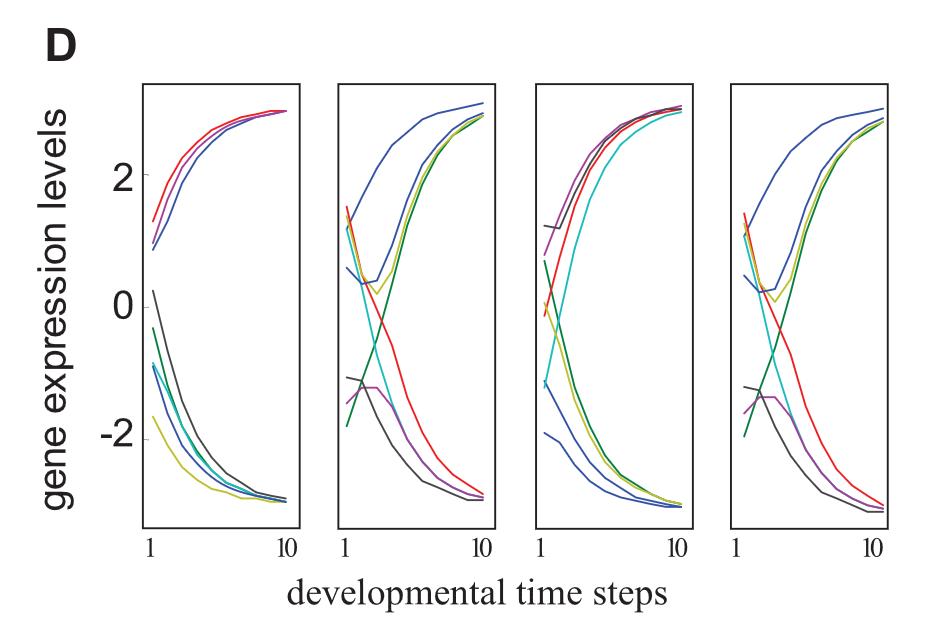
\includegraphics[width=0.9\linewidth]{orig_img/fig2d.png}
        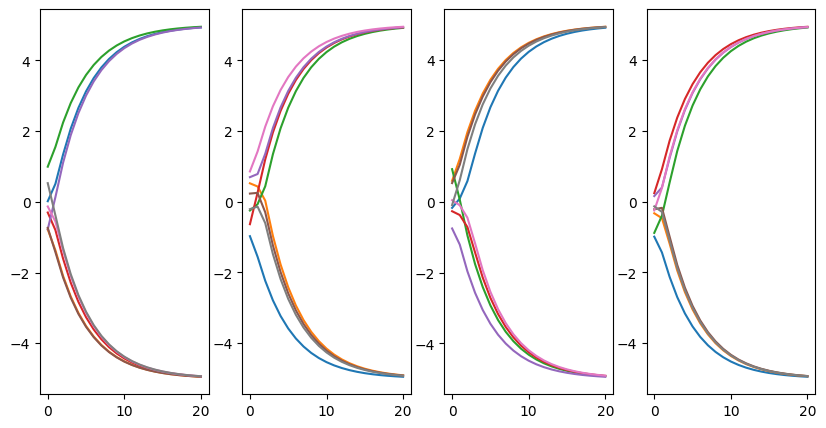
\includegraphics[width=0.9\linewidth]{img/fig2d.png}
        \caption{The constituent values of $P$ over 10 developmental timesteps. On the top is the original paper. On the bottom is the reimplemented result.} \label{fig:2d}
    \end{figure}

    After training, the GRN is also capable of producing a valid phenotype given a random input genotype. Figure \ref{fig:2e} shows a selection of such phenotypes. The results are similar to those of the original paper, with the GRN producing both targets that are present in the training data. The GRN also produces the inverses of the two targets. This is to be expected, as the GRN can only produce patterns of genes relative to other genes, so cannot enforce a certain gene to be an absolute value.

    \begin{figure}[h]
        \centering
        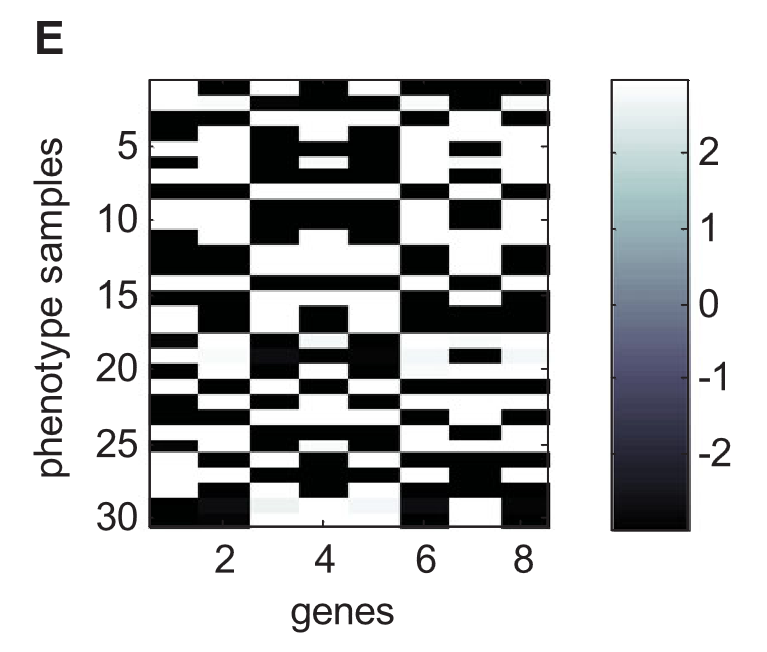
\includegraphics[width=0.45\linewidth]{orig_img/fig2e.png}
        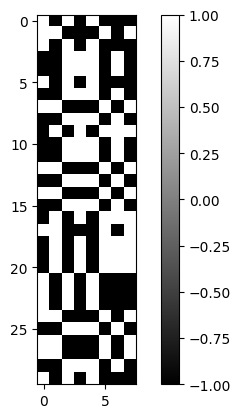
\includegraphics[width=0.45\linewidth]{img/fig2e.png}
        \caption{A bestiary of phenotypes produced using random input genotypes. On the left is the original paper. On the right is the reimplemented result.} \label{fig:2e}
    \end{figure}

    \subsection{Testing Generalisation} \label{sec:tg}
    Experiment 4 was designed to test the GRN's ability to not only remember a significantly larger number of targets than previous experiments but also explore the GRNs ability to generalize. The dataset for this experiment consisted of 8 target phenotypes, illustrated in Figure \ref{fig:4-targets}, which were designed to be highly modular. This modularity was achieved by splitting the target phenotype into 4 distinct modules, each of which could take one of two possible shapes. This presented 16 valid phenotypes, however, $50\%$ of these were omitted from the training set with the goal being that the GRN would produce some of these omitted phenotypes. This would indicate that it was learning the sub-modules, and therefore generalizing.

    \begin{figure}[h]
        \centering
        
\includegraphics[width=0.7\linewidth]{orig_img/ex4_targets.png}
        \caption{Eight target phenotypes, taken from \cite{original-paper}} \label{fig:4-targets}
    \end{figure}

    The parameters that were used in this experiment are listed in Table \ref{tbl:ex-g-param}.
    \begin{table}[h]
        \centering
        \begin{tabular}{l|l}
        Parameter & Value \\ \hline
        $G$ Mutations & Uniform[-0.1:0.1] \\
        $B$ Mutations & Uniform[-0.0067:0.0067] \\
        Generations & 3500000 \\
        Target Switch Each & 25000 \\
        $\tau_1$ & 1.0 \\
        $\tau_2$ & 0.2 \\
        $t_{final}$ & 10
        \end{tabular}
        \caption{The parameters of the generalization experiment.} \label{tbl:ex-g-param}
    \end{table}

    Figure \ref{fig:4b-orig} demonstrates a set of phenotypes produced by supplying a trained GRN with random input genotypes, taken from the original work. Figure \ref{fig:4b} presents a reproduction of this diagram implemented by this paper. In both diagrams, there are phenotypes from both the training subset of 8, but also from the 8 target phenotypes that are valid but not present in the training set. This implies that generalization is taking place.

    \begin{figure}[h]
        \centering
        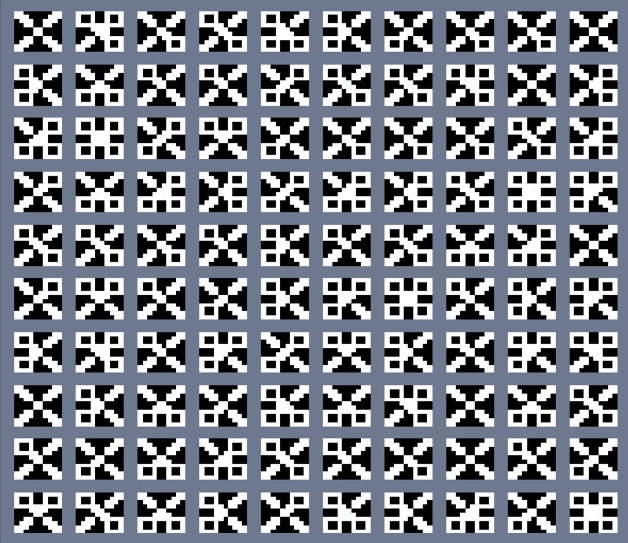
\includegraphics[width=0.7\linewidth]{orig_img/fig4b.png}
        \caption{Bestiary of genotypes from the original paper.} \label{fig:4b-orig}
    \end{figure}

    \begin{figure}[h]
        \centering
        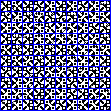
\includegraphics[width=0.7\linewidth]{img/fig4b.png}
        \caption{Bestiary of genotypes reimplemented to the specification of the original paper.} \label{fig:4b}
    \end{figure}

    \section{Extension}
    The previously described model of a GRN provides a significant abstraction of the concept of mutations, by modeling a mutation as a small change of the value of the weight between genes. However, this method ignores two other important types of mutation: enabling and disabling connections, and inverting connections.

    When a connection in the GRN is disabled, it maintains its weight but does not contribute to the development of a genotype. However, in the future, this connection may be re-enabled to restore the original weight. This is analogous to recessive genes in biology, where a gene may still exist but is not expressed in the phenotype of a creature. However, that gene may be re-enabled in a descendant of that creature, where it may once again be useful.
    
    Inverting a connection entails reversing the influence of a connection, or in the context of the mathematical model, multiplying the connection by $-1$. This provides the evolutionary process with the ability to quickly reverse the influence of a connection, and therefore the influence that one gene in the genotype has on another. This mutation abstraction has biological parallels with repressor and activator genes, which are the mechanism of GRNs for genes to control the expression level of each other. Where small incremental mutations such as those implemented by the original work may represent a change in the concentration of a produced activator or repressor, an inversion mutation may signify a switch from a gene producing a repressor to an activator, or vice versa.

    This paper presents an extension to the original model to implement these new mutation types and hypothesizes the effects of including these. The new mutations are subsequently tested in-depth, and a detailed analysis is given based on the results.

    \subsection{Goals and Hypothesis}
    Prior to presenting the hypothesis, it is important to understand one of the major factors which hinders generalization. Generalization entails learning the underlying patterns of the phenotype, in contrast to memorizing all of the genotypes present in the training set. Generalization is improved when the GRN contains as few connections as possible to represent the dataset, as this means that unimportant connections are not present. An unimportant connection contributes a very small amount to the fitness of the produced phenotype when tested on phenotypes within the training set. However, the effect of unimportant connections on new phenotypes produced from unseen data is uncertain - even though the connection was unimportant in the training data, it may make a significant difference to this new unseen data. A safe method to deal with these unimportant connections is to set them to 0, so that no matter the input, they cannot affect the result of the GRN. However, using just small delta mutations, the value of these unimportant connections may drift to high values. This is the reason that L2 normalization has been used in previous work to encourage these connections which contribute very little to fitness to return to 0 \cite{advanced-paper}.

    The following experiments aim to demonstrate the importance of the proposed types of mutation, and to present evidence for the following hypotheses:

    \begin{enumerate}
        \item The new mutation style on the GRN provides it with a fast method to disable unimportant connections. This may allow the GRN to generalize faster by using the new mutation style when compared to just simple delta mutations. However, this effect may only present itself when paired with L2 normalization to introduce pressure to remove unimportant connections.
        \item The GRN may find local optima easier to escape due to the ability for flip connections to occur, enabling much larger changes in its behavior. One of the common issues with a trained GRN is that single pixels may be confidently expressed as the incorrect color. It may be simpler for the GRN to flip these when a weight inversion is possible.
    \end{enumerate}

    \subsection{Model}
    The aims of producing a model for the updated GRN were two-fold. Firstly, the extended model should introduce as little extra complexity as possible, which would not only maintain fast simulation times but also ensure the model would not stray too far from its biological inspiration. Secondly, the model should maintain maximum similarities to the original, maintaining easy comparisons between the structure and performance of the two.

    The presented model, formalized in Equations \ref{eq:extenda} and \ref{eq:extendb}, fulfills both of these requirements. In Equation \ref{eq:extendb}, the $*$ symbol represents element-wise matrix multiplication, the matrix $B_s$ is the sign matrix, and $B_m$ denotes the magnitude matrix. The sign matrix contains values in the set $\{-1,0,1\}$, however, the magnitude matrix may contain any values. All other symbols hold the same meaning as those in Equation \ref{eq:origp}.

    \begin{equation} \label{eq:extenda}
        P(1) = G
    \end{equation}
    \begin{equation} \label{eq:extendb}
        P(t+1) = P(t) + \tau_1 \sigma ((B_s * B_m) P(t)) - \tau_2 P(t)
    \end{equation}

    Mutations on this model are applied with a different process to that of the original. First, the matrix to mutate is randomly chosen with a probability that heavily favors the matrix $B_m$. If $B_m$ was chosen, mutations are applied as described in the original model. However, if $B_s$ is chosen to be mutated, a random cell of the matrix is changed to a value chosen uniformly from the set $\{-1,0,1\}$, irrespective of what the cell's value was before.

    By extending mutation to include $B_s$, the expected magnitude of change in mutation may significantly increase. To counteract this, it is necessary to reduce the rate of mutation on $B_m$. Equation \ref{eq:rate-of-sign} presents a method to find the correct value for maximum uniform mutations on $B_m$ ($m_{ex}$) when given values for the probability of mutating $B_s$ ($p$) and an equivalent mutation rate on the un-extended GRN ($m_{orig}$). Equation \ref{eq:rate-of-sign} was derived based on the assumptions that the expected change of weight of a small uniform mutation is its probability divided by 2, and the expected change of a $B_s$ mutation is $\frac{8}{9}$.

    \begin{equation}
        m_{ex} = \frac{m_{orig} - \frac{16}{9}p}{1-p}
        \label{eq:rate-of-sign}
    \end{equation}

    \section{Extension Results}

    The primary motivation behind the introduction of this extension was to increase the generalization capability of the GRN, by providing a simple mutation to disable unnecessary connections. To measure the ability of the GRN to generalize, a new metric is presented: Proportion of Unique Classes Produced (PUCP). This metric represents what proportion of the possible correct classes for a given dataset can be produced by the GRN when provided with random input genotypes. A phenotype is defined as correct if all of its genes have the same sign as the target. Even though this appears to be a weak assumption, where genes may not be significantly different from zero, in practice, all genes in the resulting genotype take either very high or low values.

    The following experiments are all performed on the stalks dataset from Section \ref{sec:tg}. This dataset provides 8 target phenotypes, however, these only represent 50\% of the possible combinations of the 4 corner modules. The PUCP metric is calculated using all 16 possible combinations of the different corner modules. This means that if a GRN achieves a PUCP metric of larger than 0.5, the GRN must be generalizing, as it produces more valid phenotypes than are present in the training set.

    The secondary metric used to evaluate the GRNs is called Proportion of Productions Valid (POPV), which represents the proportion of phenotypes produced by the GRN, when given random input genotypes, that are present in the set of all possible phenotypes. A score of 0.25 POPV means that 25\% of the time, the GRN produces genotypes that are part of the set of valid genotypes.

    In the following experiments, various PUCP and POPV graphs are displayed. However, the graphs do not show the raw metrics, but rather a version of the metrics smoothed using a mean window function. This is important for the legibility of the graphs, as in their raw form, are extremely noisy due to the constant changing of target phenotypes. To reduce this noise further, each line on each graph displays the mean metric over 20 repeat runs. When present, a shaded area around each line denotes the standard deviation.

    \subsection{Training without L2}

    The first extension experiment aims to quantify the effect of a mutation mask on the performance of the GRN. This experiment was configured in a similar fashion to experiment 4, with the parameters displayed in Table \ref{tbl:exex1-param}.

    \begin{table}[h]
        \centering
        \begin{tabular}{l|l}
        Parameter & Value \\ \hline
        $G$ Mutations & Uniform[-0.1:0.1] \\
        $B$ Mutations & Uniform[-0.0067:0.0067] \\
        $B_m$ Mutations & Uniform[-0.0058:0.0058] \\
        $B_s$ Mutation chance & 0.0005 \\
        Generations & 3500000 \\
        Target Switch Each & 25000 \\
        $\tau_1$ & 1.0 \\
        $\tau_2$ & 0.2 \\
        $t_{final}$ & 10 \\
        $L2$ & 0.0 \\
        \end{tabular}
        \caption{The parameters of this experiment.} \label{tbl:exex1-param}
    \end{table}

    Figures \ref{fig:ex-A} and \ref{fig:ex-A2} show the results of this test. In both graphs, it is clear that the dense (original) model outperformed the masked dense (extended) model. However, in Figure \ref{fig:ex-A}, the final PUCP scores of both models tend toward the same value, indicating that both models were able to generalize to the same degree.
    
    The same cannot be said for Figure \ref{fig:ex-A2}, which shows that not only was the original model faster to reach higher values, but also that it settled on a slightly higher score by the end of the training, meaning that the original model was more likely to produce valid results.

    In both Figure \ref{fig:ex-A} and Figure \ref{fig:ex-A2}, the standard deviation in the PUCP and POPV scores is significantly lower towards the end of training for the dense network than that of the masked dense one. This indicated that the masked dense network may reduce repeatability and predictability when in this scenario.

    \begin{figure}[h]
        \centering
        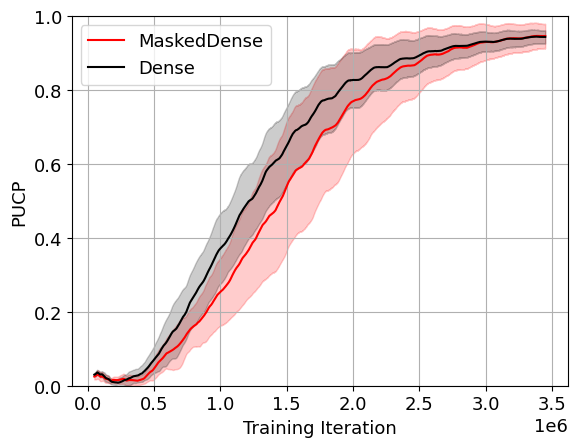
\includegraphics[width=0.7\linewidth]{ex-img/final-nol2-pucp.png}
        \caption{PUCP of the original model compared to that of the new model.} \label{fig:ex-A}
    \end{figure}

    \begin{figure}[h]
        \centering
        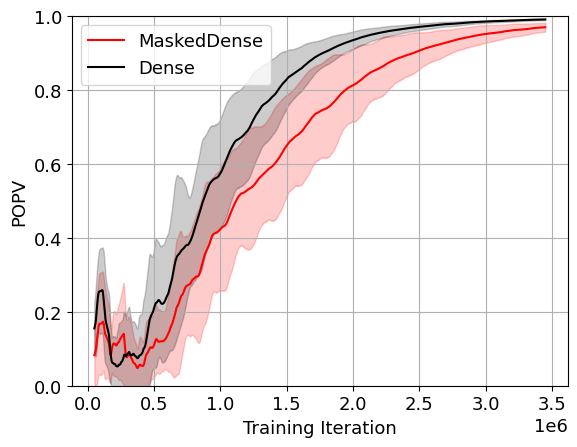
\includegraphics[width=0.7\linewidth]{ex-img/final-nol2-popv.png}
        \caption{POPV of the original model compared to that of the new model.} \label{fig:ex-A2}
    \end{figure}

    \subsection{Training with L2}

    As stated in the hypothesis, there may be no pressure for the new mutation strategy to disable unimportant connections unless a normalization factor such as L2 normalization was applied during training. For this reason, the above tests were repeated, but with both methods having an L2 normalization factor of 5. The L2 normalization value was calculated according to Equation \ref{eq:l2}, where taking the power of a matrix denotes an element-wise power. The L2 value was then subtracted from each GRN's fitness to obtain its adjusted fitness.

    \begin{equation}
        val_{l2} = l2*sum(B^2)
        \label{eq:l2}
    \end{equation}

    Figures \ref{fig:ex-B} and \ref{fig:ex-B2} illustrate the results obtained from this test. In the same fashion as the previous experiment, the POPV score attained by the masked dense GRN was slightly lower than that of the dense GRN. However, when compared to the experiment where no normalization was present, it is clear that both GRNs' POPV scores are lower by almost $0.15$.
    
    The more promising results are illustrated in Figure \ref{fig:ex-B}, which shows that the PUCP score for the masked GRN ends up at a higher value than that of the dense network despite lagging in performance for much of the training. In addition to this, the standard deviation for masked dense is lower than not only that of the dense GRN but also when compared to the masked dense GRN in Figure \ref{fig:ex-A}. Interestingly, the L2 normalization had the opposite effect on the dense GRN, increasing its standard deviation when L2 normalization was applied.

    \begin{figure}[h]
        \centering
        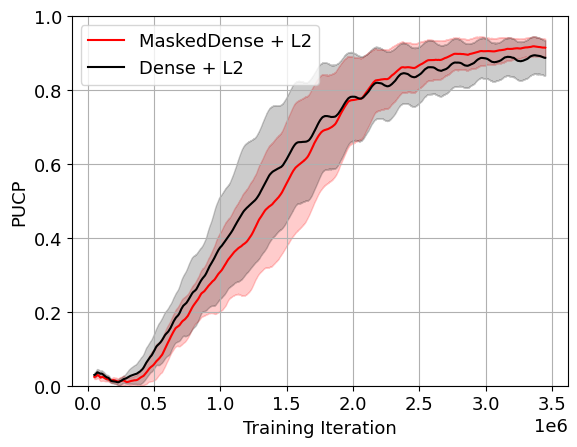
\includegraphics[width=0.7\linewidth]{ex-img/final-l2-pucp.png}
        \caption{PUCP of the original model compared to that of the new model.} \label{fig:ex-B}
    \end{figure}

    \begin{figure}[h]
        \centering
        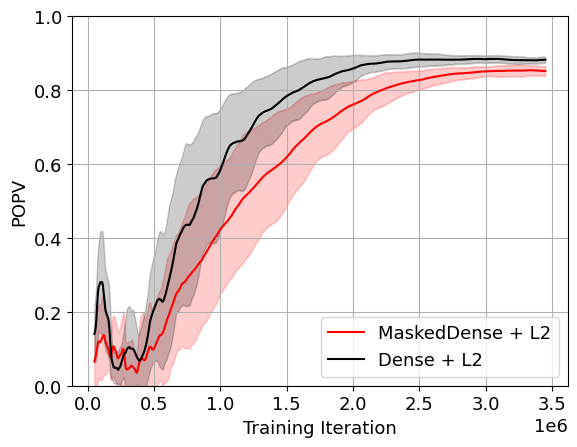
\includegraphics[width=0.7\linewidth]{ex-img/final-l2-popv.png}
        \caption{POPV of the original model compared to that of the new model.} \label{fig:ex-B2}
    \end{figure}

    \subsection{Comparison to Hebbian}
    To verify that the new method of mutation still tends towards the weights achieved through Hebbian learning, the matrix $B$ was examined. Figure \ref{fig:ex-weights} compares the weights achieved through these two methods. It is clear from this figure that the learned weights follow the same pattern as those from Hebbian learning, albeit with a higher degree of noise.

    \begin{figure}[h]
        \centering
        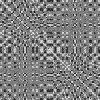
\includegraphics[width=0.45\linewidth]{ex-img/masked_weights.png}
        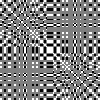
\includegraphics[width=0.45\linewidth]{ex-img/hebb_weights.png}
        \caption{The weights of $B$ ($B_mB_s$) after training. On the left are the trained weights, and on the right are the Hebbian weights.} \label{fig:ex-weights}
    \end{figure}

    It is also important to inspect the mask of the evolved GRN, to determine if it is having a significant impact on the output. Figure \ref{fig:ex-mask} provides a visualization of the mask after the evolutionary process is complete. The high number of white pixels, which denote a value of one, is likely since the matrix starts initialized as all ones. Interestingly, the pattern of grey pixels, denoting zero, does not seem to mirror the grey pixels in the output image but instead seems to be random. The GRN has certainly made use of the ability to quickly flip gene connections, demonstrated by the frequent black pixels in the image.

    \begin{figure}[h]
        \centering
        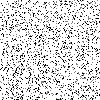
\includegraphics[width=0.45\linewidth]{ex-img/masked_mask.png}
        \caption{The values of $B_s$ after training.} \label{fig:ex-mask}
    \end{figure}

    \section{Evaluation of Extension}
    The extension experiments showed that in most scenarios, the new mutation style hindered the progress of the GRN. One possible reason for this is that the new mutation style may still have allowed mutations to happen too quickly, even with the reduced original learning rate and low probability. The specific problem presented in this paper is extremely sensitive to the relative learning rate of the GRN when compared to the initial genotype. A possible future solution to this would be to also apply the new mutation style to the genotype, meaning there would be no relative change in learning rate between the two components.
    
    After examining the mask matrix of the GRN, it is clear that there is no pattern present in the mask. One of the key reasons for including the mask matrix was to easily allow the GRN to completely disable unimportant connections, however, this did not significantly occur in these experiments. A solution to this problem may be to apply normalization to the mask matrix, instead of the premultiplied matrix. This would encourage the network to disable as many connections as possible, as opposed to providing pressure to reduce the magnitude of all of the weights.

    These experiments broadly failed to prove both hypotheses. It was extremely difficult to determine if the new mutation style was able to generalize more effectively than the original, as the original was already extremely effective at generalization. However, when strong normalization was applied, the extended mutation strategy was able to outperform the original in terms of generalization. Future work may repeat the presented experiments, but with a dataset that the original model finds more difficult to generalize on, thus providing room for improvement. The second hypothesis was also not proven, as the new mutation style did not significantly increase the ability of the GRN to escape local optima. However, this hypothesis was based on heuristic evidence found by examining the outputs of single runs. It became clear throughout the process that the assumption that the GRN frequently became stuck in local optima was incorrect, therefore preventing the hypothesis from being proven. However, the author still believes that the new mutation style may be able to help the GRN escape local optima and that this should be tested in future work.
    
    \section{Conclusion}
    This study has not only shown the reproducibility of the results obtained by R. Watson et al \cite{original-paper} but has also contributed some valuable insights into iterative improvements on the model of a GRN.

    The reimplementations of the original paper's models and experiments have firmly established that, in the specific scenarios tested, evolution on a GRN is equivalent to Hebbian learning, suggesting that evolution may provide a more 'intelligent' method of learning than originally thought.

    The extension to the original model provided the evolutionary process with the ability to quickly and invert the influence of connections. The results of the experiments show that in many scenarios, the old mutation style outperforms the original, however, when paired with L2 normalization, the new mutation style can prevail.

    Overall, this paper has shown that the model of a GRN is a powerful tool for learning and generalizing from data and that the addition of new mutation types may potentially increase the GRN's ability to generalize and escape local optima. It has also presented a new style of mutations that may not be exclusively applied to GRNs, but may also be useful in other evolutionary machine learning scenarios. Although the hypotheses were not proven, this paper has provided a solid foundation for future work in this area.

    \bibliography{report}


\end{document}